\chapter{Task 5}
In this chapter task 4 was continued, the aim was now to attempt to steer the irregular spaced array with an excitation current $I_n  = A_n e^{j\Phi_n}$. This was illustrated by computing a MATLAB function which constructed the excitation current as a function of array antenna positions $\{r_i\}_{i=1}^N$  and steering angles $\theta_0, \phi_0$.

To begin the theory regarding a steered array antenna  and phase shifts will be presented. Then the results from the computations will be presented. 

\section{Theory}
As mentioned before array antennas are good to use because they can be steered, i.e. every element is directed according to a steering vector with fixed angles $\theta_0$ and $\phi_0$. The difference in phase (phase shift) between two elements are $\Phi_{n, n-1}$, which is the length difference of the two elements times the wave vector k. Consider now the spherical coordinates 
\begin{equation}
\hat{r} = sin\theta cos\phi \hat{x} + sin\theta sin\phi \hat{y} + cos\theta \hat{z},
\end{equation}
if the array antenna is steered in a direction $\theta_0$ and $\phi_0$ and the elements of the array are placed in positions $\{\mathbf{r}_i \}_{i=1}^N$ we may project the positions on the steering vector as 
\begin{align}
& d_n = \mathbf{r}_n \cdot \hat{r} = (x_n\hat{x}+ y_n\hat{y} + z_n\hat{z}) (sin\theta_0 cos\phi_0 \hat{x} + sin\theta_0 sin\phi_0 \hat{y} + cos\theta_0 \hat{z})= \\
& sin\theta_0 cos\phi_0 x_n + sin\theta_0 sin\phi_0 y_n + cos\theta_0 z_n.
\end{align}
An illustration of the projection can be viewed in figure \ref{fig:farfieldProjetion}.
\begin{figure}
\centering
\includegraphics[width=0.7\linewidth]{pictures/farfieldProjetion}
\caption{This figure shows how a vector can be projected onto another in the far field region of antennas. This figure was obtained from \cite{kildal2000foundations}}
\label{fig:farfieldProjetion}
\end{figure}
The difference in length between two arbitrary elements in space is thus
\begin{align}
& d_{n,n-1} = |d_n-d_{n-1}| = |\mathbf{r}_n \cdot \hat{r} -\mathbf{r}_{n-1} \cdot \hat{r}| =\\
& | sin\theta_0 cos\phi_0 (x_n -x_{n-1}) + sin\theta_0 sin\phi_0 (y_n -y_{n-1})  + cos\theta_0 (z_n -z_{n-1}) |.
\end{align}
The phase difference  between two elements subsequently  be computed as 
\begin{equation}
\Phi_{n, n-1} = kd_{n,n-1} = \frac{2\pi}{\lambda} | sin\theta_0 cos\phi_0 (x_n -x_{n-1}) + sin\theta_0 sin\phi_0 (y_n -y_{n-1})  + cos\theta_0 (z_n -z_{n-1}) |. 
\end{equation}
However, the actual phase difference that is interesting to compute is the phase difference with respect to the steering vector for each element
\begin{equation}
\Phi_{n, 0} = kd_{n,0} = \frac{2\pi}{\lambda} | sin\theta_0 cos\phi_0 (x_n) + sin\theta_0 sin\phi_0 (y_n)  + cos\theta_0 (z_n)|. 
\end{equation}

It was assumed for this task that the amplitude of the current was 1 A and that the positions are given in $ m \lambda$. Thus the excitation current can be computed to be 
\begin{equation}
I_n = e^{j\Phi_{n, 0}} =e^{ \frac{2\pi}{\lambda} | sin\theta_0 cos\phi_0 (x_n) + sin\theta_0 sin\phi_0 (y_n)  + cos\theta_0 (z_n)| }.
\end{equation}\cite{kildal2000foundations}


\section{Results}
The MATLAB scripts for this section are presented in section \ref{section:task5.m}. The result of the phase of the current was plotted in figure \ref{task5:phase} for an equispaced and irregular array. The amplitude of the current was chosen not to be plotted since the amplitude of the excitation current was assumed to be unity.

\begin{figure}[h]
\centering
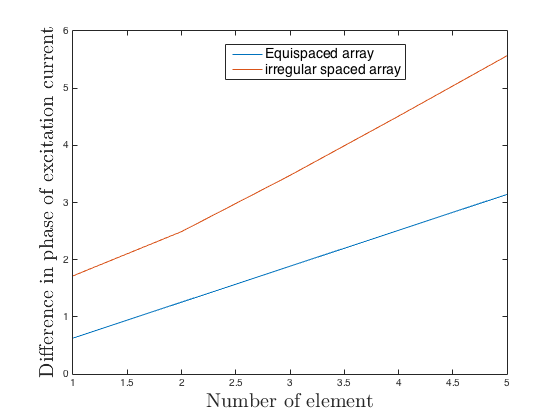
\includegraphics[scale=0.6]{/Users/marikasvensson/Documents/MATLAB/MicroProject/finished/task5/excitationCurrent.png}
\caption{This figure shows the phase with respect to the steering vector of the excitation current as a function of element positions and steering direction $\theta_0 = \pi/3$rad and $\phi_0 = \pi/2$rad }
\label{task5:phase}
\end{figure}

The phase difference between the elements were also computed an plotted in figure \ref{task5:phaseNeigh}.

\begin{figure}[h]
\centering
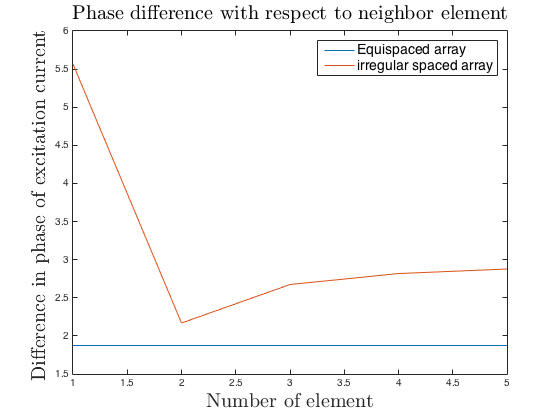
\includegraphics[scale=0.6]{/Users/marikasvensson/Documents/MATLAB/MicroProject/finished/task5/excitationCurrentNeighbour.png}
\caption{This figure shows the phase of the excitation current with respect to the neighbor as a function of element positions and steering direction $\theta_0 = \pi/3$rad and $\phi_0 = \pi/2$rad }
\label{task5:phaseNeigh}
\end{figure}




\begin{comment}
\begin{equation}
\Psi_n = \frac{2\pi}{\lambda}( d_n sin(\theta_0) )
\end{equation}
where $\theta_0$ is the scanning angle and $\d_n = |\mathbf{r}_n - \mathbf{r}_{n-1}|$ is the intermediate distance between element n and n-1. 



The total phase shift for an element should then be 
\begin{equation}
\phi_n^{tot} = \sum_{i=1}^n \Psi_i.
\end{equation} 
% Calculatin the amplitude??
For the amplitude we may use the formula we will set the current amplitude to 1. 





A steering vector $\mathbf{v(k)}$ is the representation of the phase delay that each element in the array antenna has, which is defined as 

\begin{equation}
\mathbf{v(k)}=[e^{-j\mathbf{k}\cdot\mathbf{r}_1} ... e^{-j\mathbf{k}\cdot\mathbf{r}_N} ]
\end{equation}
We can write an output function Y as 

\begin{equation}
R_A = R(\theta, \phi) \sum_i w_ie^{-j\mathbf{k}\cdot\mathbf{r}_i} = G(\theta, \phi)AF
\end{equation}
where

\begin{equation}
AF = \mathbb{w}^T\mathbf{v(k)}
\end{equation}
and  $R(\theta, \phi)$
\if
\end{comment}
